\documentclass[10pt]{beamer}

\usetheme{Oxygen}
\usepackage{thumbpdf}
\usepackage{wasysym}
\usepackage{ucs}
\usepackage[utf8]{inputenc}
\usepackage{pgf,pgfarrows,pgfnodes,pgfautomata,pgfheaps,pgfshade}
\usepackage{verbatim}
\usepackage{tikzsymbols}

\usepackage{ragged2e} % maneja la alineación del documento
\usepackage[spanish]{babel} % Títulos en español
\usepackage[utf8]{inputenc}
%\usepackage[latin1]{inputenc} % Caracteres con acentos.
\usepackage{graphicx} % Soporte para gráficos
\usepackage[none]{hyphenat} % indica a LaTeX que no debe hacer partición de palabras
\usepackage[T1]{fontenc} % manejo de fuentes
\usepackage{array}
\usepackage{amsmath}
\usepackage{amssymb}
\usepackage{float}
%\usepackage{ra  gged2e}
\usepackage [all]{xy}
\usepackage{lmodern}
\usepackage{multirow}
\usepackage{multicol}
\usepackage{tikz}
\usepackage{listings}

\lstset{keywordstyle=\color{blue}, 
commentstyle=\color{gray!90}, 
basicstyle=\ttfamily\small, 
columns=fullflexible, 
breaklines=true,
linewidth=\textwidth, 
backgroundcolor=\color{gray!20}, 
basewidth={0.5em,0.4em}, 
literate={á}{{\'a}}1 {ñ}{{\~n}}1 {é}{{\'e}}1 {ó}{{\'o}}1 {º}{{\textordmasculine}}1, 
showstringspaces=false}



\setbeamersize{text margin left=9mm,text margin right=7mm} 


\pdfinfo
{
  /Title       (Maestría en Analítica e Inteligencia de Negocios)
  /Creator     (TeX)
  /Author      (Orlando Joaqui-Barandica)
}


\title{Maestría en Analítica e Inteligencia de Negocios}
\subtitle{Clase: Series de tiempo y pronóstico}
\author{PhD. St. Orlando Joaqui-Barandica} 
\institute{Universidad del Valle}
\date{2021}

\sloppy % Indica a LaTex que debe minimizar el corte de las palabras para pasar de una línea a otra
\justifying % justificar todo el documento


\begin{document}

\frame{\titlepage}


\begin{frame}
  \frametitle{Contenido}
  \tableofcontents[hidesubsections]
\end{frame}

\AtBeginSection[]
{
  \frame<handout:0>
  {
    \frametitle{Contenido}
    \tableofcontents[currentsection,hideallsubsections]
  }
}

    
\AtBeginSubsection[]
{
  \frame<handout:0>
  {
    \frametitle{Contenido}
    \tableofcontents[sectionstyle=show/hide,subsectionstyle=show/shaded/hide]
  }
}

\newcommand<>{\highlighton}[1]{%
  \alt#2{\structure{#1}}{{#1}}
}

\newcommand{\icon}[1]{\pgfimage[height=1em]{#1}}



%%%%%%%%%%%%%%%%%%%%%%%%%%%%%%%%%%%%%%%%%
%%%%%%%%%% Content starts here %%%%%%%%%%
%%%%%%%%%%%%%%%%%%%%%%%%%%%%%%%%%%%%%%%%%

\section{Introducción}


\begin{frame}
\frametitle{¿Qué se puede pronosticar?}

Se requieren \highlighton{pronósticos} en muchas situaciones:

\vspace{4mm}

\begin{itemize}
\justifying
\item Decidir si se construirá otra planta de generación de energía en los próximos cinco años requiere pronósticos de la demanda futura.
\vspace{3mm}
\item Programar el personal en un centro de llamadas la próxima semana requiere pronósticos de volúmenes de llamadas.
\vspace{3mm}
\item Almacenar un inventario requiere pronósticos de los requisitos de stock. Se pueden requerir pronósticos con varios años de anticipación (para el caso de inversiones de capital), o solo unos minutos antes (para el enrutamiento de telecomunicaciones). 

\end{itemize}



\end{frame}


%%%%%%%%%%%%%%%%%%%%%%%%%%%%%%%%%%%%%%%%%%%%%%%%%%%%%%%%%%%%




\begin{frame}
\frametitle{¿Qué se puede pronosticar?}

\begin{center}
\textit{Cualesquiera que sean las circunstancias o los horizontes de tiempo involucrados, el pronóstico es una ayuda importante para una planificación efectiva y eficiente.}
\end{center}

\vspace{4mm}

\begin{minipage}{0.3\textwidth}
\pause
\begin{figure}
\begin{center}
    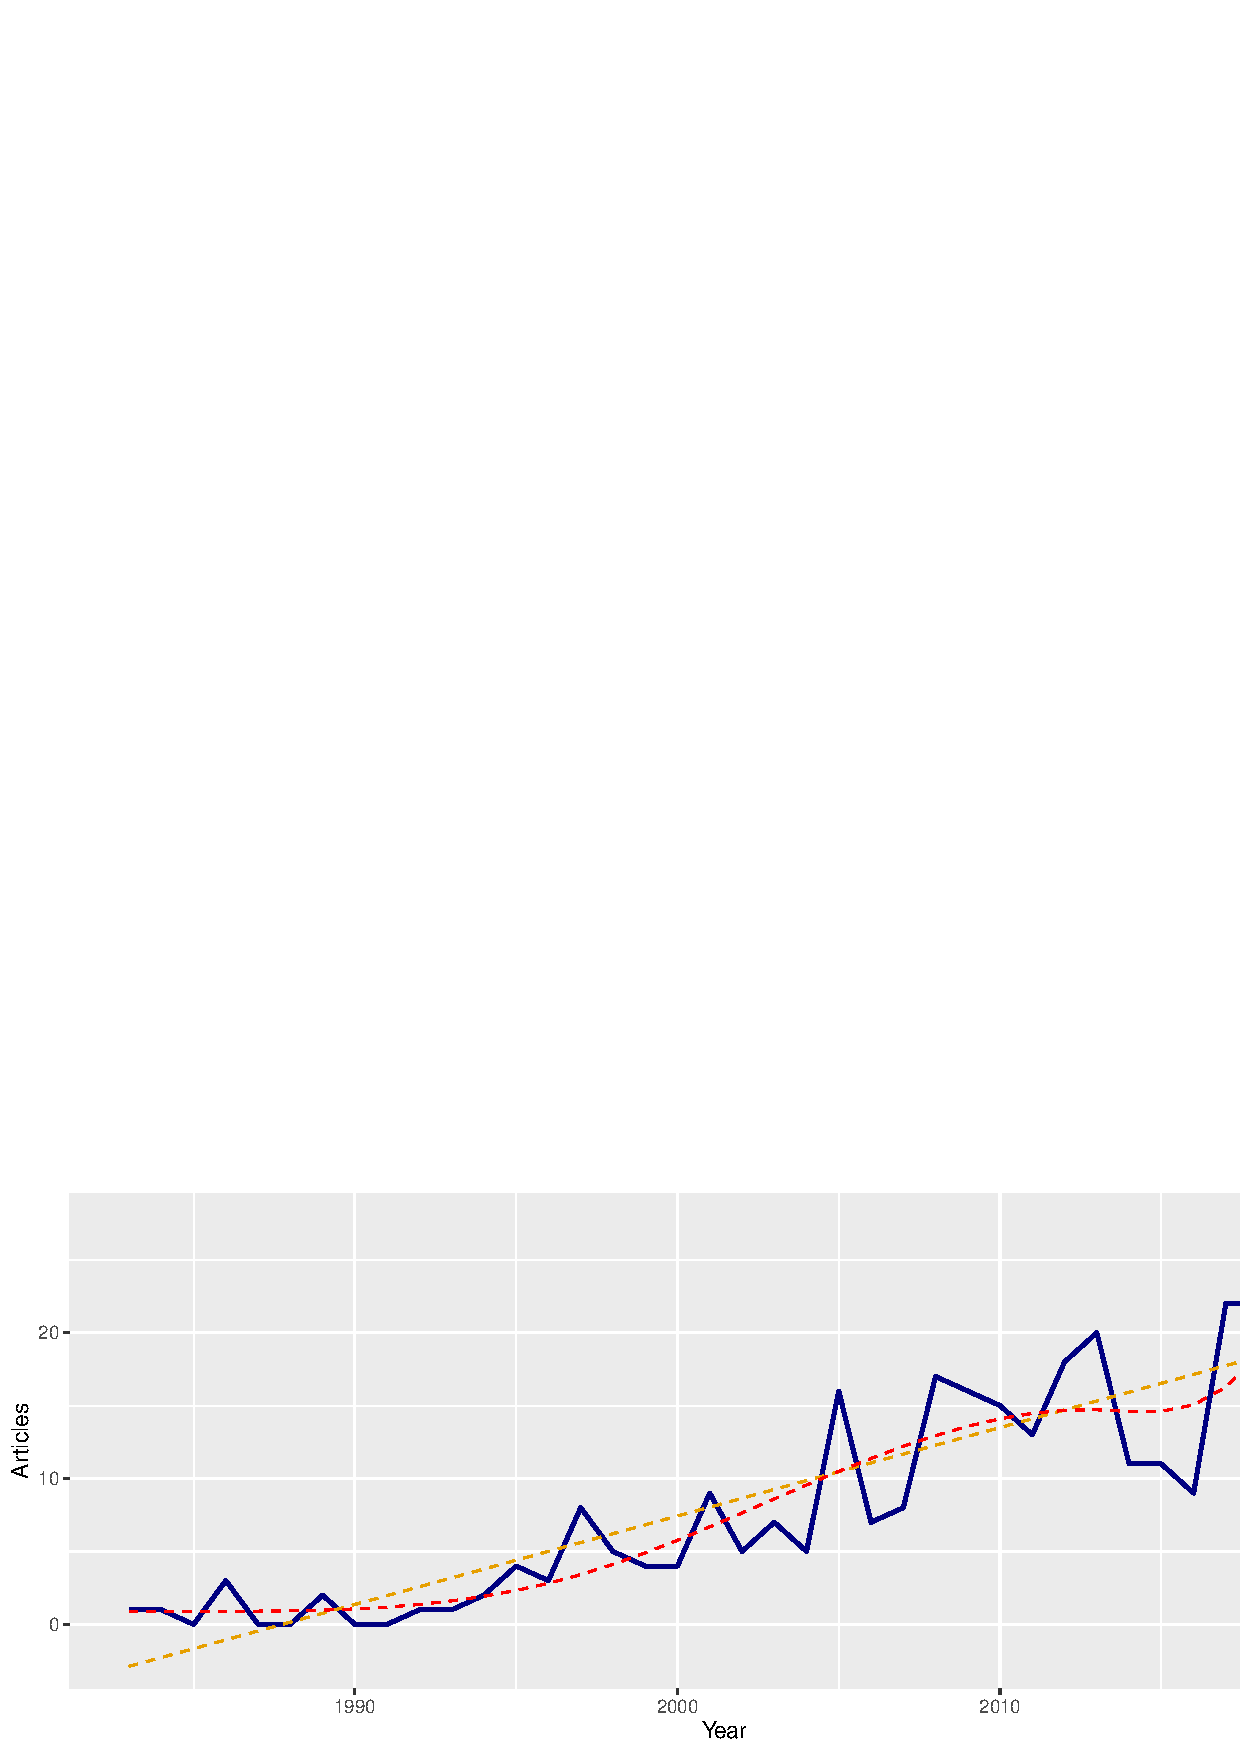
\includegraphics[width=0.9\textwidth]{Imagen1.JPG}
\end{center}
\end{figure}
\end{minipage}
\begin{minipage}{0.3\textwidth}
\pause
\begin{figure}
\begin{center}
    \includegraphics[width=0.9\textwidth]{Imagen2.JPG}
\end{center}
\end{figure}
\end{minipage}
\begin{minipage}{0.3\textwidth}
\pause
\begin{figure}
\begin{center}
    \includegraphics[width=0.9\textwidth]{Imagen3.JPG}
\end{center}
\end{figure}
\end{minipage}
\begin{minipage}{0.3\textwidth}
\pause
\begin{figure}
\begin{center}
    \includegraphics[width=0.9\textwidth]{Imagen4.png}
\end{center}
\end{figure}
\end{minipage}
\begin{minipage}{0.34\textwidth}
\pause
\begin{figure}
\begin{center}
    \includegraphics[width=0.9\textwidth]{Imagen5.png}
\end{center}
\end{figure}
\end{minipage}
\begin{minipage}{0.34\textwidth}
\pause
\begin{figure}
\begin{center}
    \includegraphics[width=0.9\textwidth]{Imagen6.JPG}
\end{center}
\end{figure}
\end{minipage}



\end{frame}


%%%%%%%%%%%%%%%%%%%%%%%%%%%%%%%%%%%%%%%%%%%%%%%%%%%%%%%%%%%%


%%%%%%%%%%%%%%%%%%%%%%%%%%%%%%%%%%%%%%%%%%%%%%%%%%%%%%%%%%%%




\begin{frame}
\frametitle{Predicción de series de tiempo}

Al pronosticar datos de series temporales, el objetivo es estimar cómo la secuencia de observaciones continuará en el futuro.


\begin{figure}
\begin{center}
    \includegraphics[width=0.6\textwidth]{Imagen7.JPG}
\end{center}
\end{figure}

\begin{itemize}
\scriptsize
\item Observe cómo los pronósticos capturaron el patrón estacional visto en los datos históricos y lo replicaron durante los próximos dos años. 

\item La región sombreada muestra intervalos de predicción del 80\%. Es decir, se espera que cada valor futuro se encuentre en la región sombreada con una probabilidad del 80\%.
\end{itemize}


\end{frame}


%%%%%%%%%%%%%%%%%%%%%%%%%%%%%%%%%%%%%%%%%%%%%%%%%%%%%%%%%%%%




\begin{frame}
\frametitle{Predicción de series de tiempo}

Al pronosticar datos de series temporales, el objetivo es estimar cómo la secuencia de observaciones continuará en el futuro.

\vspace{4mm}

\begin{figure}
\begin{center}
    \includegraphics[width=0.8\textwidth]{Imagen8.JPG}
\end{center}
\end{figure}



\end{frame}


%%%%%%%%%%%%%%%%%%%%%%%%%%%%%%%%%%%%%%%%%%%%%%%%%%%%%%%%%%%%


\begin{frame}
\frametitle{Predicción de series de tiempo}

Los métodos de predicción de series de tiempo más simples utilizan solo información sobre la variable a pronosticar y no intentan descubrir los factores que afectan su comportamiento. 

\vspace{4mm}

Por lo tanto, extrapolarán tendencias y patrones estacionales, pero \highlighton{ignorarán} toda otra información, como iniciativas de marketing, actividad de la competencia, cambios en las condiciones económicas, etc.

\begin{center}
\highlighton{Los modelos de series de tiempo utilizados para el pronóstico incluyen modelos de descomposición, modelos de suavizado exponencial y modelos ARIMA}
\end{center}

\end{frame}


%%%%%%%%%%%%%%%%%%%%%%%%%%%%%%%%%%%%%%%%%%%%%%%%%%%%%%%%%%%%




\begin{frame}
\frametitle{Pasos para el pronóstico}


\begin{enumerate}
\item[1.] \textbf{Paso 1: Definición del problema.} \\
La definición cuidadosa del problema requiere una comprensión de la forma en que se utilizarán los pronósticos, quién los requiere y cómo se ajusta la función de pronóstico dentro de la organización que los requiere
\vspace{2mm}
\item[2.] \textbf{Paso 2: Recopilación de información.} \\
Siempre se requieren al menos dos tipos de información: \highlighton{\textbf{(a)}} datos estadísticos, y \highlighton{\textbf{(b)}} la experiencia acumulada de las personas que recopilan los datos y utilizan los pronósticos. 
\end{enumerate}

\end{frame}


%%%%%%%%%%%%%%%%%%%%%%%%%%%%%%%%%%%%%%%%%%%%%%%%%%%%%%%%%%%%






\begin{frame}
\frametitle{Pasos para el pronóstico}


\begin{enumerate}
\item[3.] \textbf{Paso 3: Análisis preliminar (exploratorio).}  \\
Comience siempre graficando los datos. 
\begin{itemize}
\item ¿Hay patrones consistentes? 
\item ¿Hay una tendencia significativa? 
\item ¿Es importante la estacionalidad? 
\item ¿Hay evidencia de la presencia de ciclos económicos? 
\item ¿Hay valores atípicos en los datos que deben ser explicados por aquellos con conocimiento experto? 
\item ¿Qué tan fuertes son las relaciones entre las variables disponibles para el análisis?
\end{itemize}

\end{enumerate}

\end{frame}


%%%%%%%%%%%%%%%%%%%%%%%%%%%%%%%%%%%%%%%%%%%%%%%%%%%%%%%%%%%%





\begin{frame}
\frametitle{Pasos para el pronóstico}


\begin{enumerate}
\item[4.] \textbf{Paso 4: Elección y ajuste de modelos.}  \\
El mejor modelo a utilizar depende de la disponibilidad de datos históricos, la fuerza de las relaciones entre la variable de pronóstico y cualquier variable explicativa, y la forma en que se usarán los pronósticos.
\begin{itemize}
\item Modelos de regresión
\item Métodos de suavizado exponencial
\item Modelos ARIMA de Box-Jenkins
\item Modelos de regresión dinámica
\item Pronóstico jerárquico
\item Redes neuronales y autorregresión vectorial
\item ...
\end{itemize}

\end{enumerate}

\end{frame}


%%%%%%%%%%%%%%%%%%%%%%%%%%%%%%%%%%%%%%%%%%%%%%%%%%%%%%%%%%%%





\begin{frame}
\frametitle{Pasos para el pronóstico}


\begin{enumerate}
\item[5.] \textbf{Paso 5: Uso y evaluación de un modelo de pronóstico.}  \\
Una vez que se ha seleccionado un modelo y se han estimado sus parámetros, el modelo se usa para hacer pronósticos. El rendimiento del modelo solo puede evaluarse adecuadamente después de que los datos para el período de pronóstico estén disponibles.\\
\vspace{3mm}
Se han desarrollado varios métodos para ayudar a evaluar la precisión de los pronósticos.
\end{enumerate}

\end{frame}


%%%%%%%%%%%%%%%%%%%%%%%%%%%%%%%%%%%%%%%%%%%%%%%%%%%%%%%%%%%%



\begin{frame}
\frametitle{La perspectiva del pronóstico estadístico}


\begin{center}
¿Es el pronóstico una variable aleatoria?
\end{center}

\pause
\vspace{3mm}

Lo que estamos tratando de pronosticar es desconocido (o no lo estaríamos pronosticando), por lo que podemos pensar en él como una \highlighton{variable aleatoria.}

\vspace{3mm}

Por ejemplo, las ventas totales para el próximo mes podrían tomar un rango de valores posibles, y hasta que sumemos las ventas reales al final del mes, no sabemos cuál será el valor. Entonces, hasta que sepamos las ventas para el próximo mes, es una cantidad aleatoria.


\end{frame}


%%%%%%%%%%%%%%%%%%%%%%%%%%%%%%%%%%%%%%%%%%%%%%%%%%%%%%%%%%%%




\begin{frame}
\frametitle{La perspectiva del pronóstico estadístico}



En la mayoría de las situaciones de pronóstico, la variación asociada con lo que pronosticamos se reducirá a medida que se aproxime el evento. En otras palabras, cuanto más adelante pronostiquemos, más inseguros estamos.

\vspace{3mm}

\begin{figure}
\begin{center}
    \includegraphics[width=0.6\textwidth]{Imagen10.JPG}
\end{center}
\end{figure}


\end{frame}


%%%%%%%%%%%%%%%%%%%%%%%%%%%%%%%%%%%%%%%%%%%%%%%%%%%%%%%%%%%%



\begin{frame}
\frametitle{La perspectiva del pronóstico estadístico}



La siguiente gráfica muestra intervalos de \highlighton{80\%} y \highlighton{95\%} para los futuros visitantes internacionales australianos. La línea azul es el promedio de los posibles valores futuros, que llamamos pronósticos puntuales .
\vspace{3mm}

\begin{figure}
\begin{center}
    \includegraphics[width=0.6\textwidth]{Imagen11.JPG}
\end{center}
\end{figure}


\end{frame}


%%%%%%%%%%%%%%%%%%%%%%%%%%%%%%%%%%%%%%%%%%%%%%%%%%%%%%%%%%%%




\section{Gráficos de series de tiempo}

\begin{frame}
\frametitle{Gráficos de series de tiempo}

Lo primero que debe hacer en cualquier tarea de análisis de datos es trazar los datos. Los gráficos permiten visualizar muchas características de los datos, incluidos patrones, observaciones inusuales, cambios en el tiempo y relaciones entre variables. 

\vspace{4mm}
Las características que se ven en los gráficos de los datos deben incorporarse, tanto como sea posible, en los métodos de pronóstico que se utilizarán. 


\end{frame}


%%%%%%%%%%%%%%%%%%%%%%%%%%%%%%%%%%%%%%%%%%%%%%%%%%%%%%%%%%%%



\begin{frame}[fragile]
\frametitle{Objetos ts}


Una serie temporal puede considerarse como una lista de números, junto con información sobre las veces que se registraron esos números. Esta información puede almacenarse como un \highlighton{ts objeto} en R.\\

\vspace{4mm}
Suponga que tiene observaciones anuales de los últimos años:

\begin{center}
\begin{tabular}{cc}
\hline 
Año & Obs \\ 
\hline 
2012 & 123 \\ 
2013 & 39 \\ 
2014 & 78 \\ 
2015 & 52 \\ 
2016 & 110 \\ 
\hline 
\end{tabular} 

\end{center}


\end{frame}


%%%%%%%%%%%%%%%%%%%%%%%%%%%%%%%%%%%%%%%%%%%%%%%%%%%%%%%%%%%%




\begin{frame}[fragile]
\frametitle{Objetos ts}


\lstset{language=r,label= ,caption= ,captionpos=b,numbers=none}
\begin{lstlisting}
y <- ts(c(123,39,78,52,110), start=2012)
\end{lstlisting}

\pause

\begin{verbatim}
Time Series:
Start = 2012 
End = 2016 
Frequency = 1 
[1] 123  39  78  52 110
\end{verbatim}

\pause


\lstset{language=r,label= ,caption= ,captionpos=b,numbers=none}
\begin{lstlisting}
y <- ts(c(123,39,78,52,110), start=2003, frequency=12)
\end{lstlisting}

\pause

\begin{verbatim}
     Jan Feb Mar Apr May
2003 123  39  78  52 110
\end{verbatim}



\end{frame}


%%%%%%%%%%%%%%%%%%%%%%%%%%%%%%%%%%%%%%%%%%%%%%%%%%%%%%%%%%%%






\begin{frame}[fragile]
\frametitle{Objetos ts}

La \highlighton{frecuencia} es el número de observaciones antes de que se repita el patrón estacional. Cuando se usa la ts() función en R, se deben usar las siguientes opciones.

\begin{center}
\begin{tabular}{cc}
\hline 
Datos & Frec \\ 
\hline 
Anual & 1 \\ 
Trimestre & 4 \\ 
Mensual & 12 \\ 
Semanal & 52 \\ 
\hline 
\end{tabular} 

\end{center}

\end{frame}


%%%%%%%%%%%%%%%%%%%%%%%%%%%%%%%%%%%%%%%%%%%%%%%%%%%%%%%%%%%%





\begin{frame}[fragile]
\frametitle{Gráficos de tiempo}


\lstset{language=r,label= ,caption= ,captionpos=b,numbers=none}
\begin{lstlisting}
y <- ts(c(123,39,78,52,110), start=2003, frequency=12)
plot(y)
\end{lstlisting}

\pause



\begin{figure}
\begin{center}
    \includegraphics[width=0.6\textwidth]{Imagen12.JPG}
\end{center}
\end{figure}




\end{frame}


%%%%%%%%%%%%%%%%%%%%%%%%%%%%%%%%%%%%%%%%%%%%%%%%%%%%%%%%%%%%



\begin{frame}[fragile]
\frametitle{Gráficos de tiempo}

Cargar la librería \textbf{fpp2}

\lstset{language=r,label= ,caption= ,captionpos=b,numbers=none}
\begin{lstlisting}
library(fpp2)

melsyd

\end{lstlisting}

\pause

{\scriptsize
\begin{verbatim}
Time Series:
Start = c(1987, 26) 
End = c(1992, 48) 
Frequency = 52 
         First.Class Business.Class Economy.Class
1987.481       1.912             NA        20.167
1987.500       1.848             NA        20.161
1987.519       1.856             NA        19.993
1987.538       2.142             NA        20.986
1987.558       2.118             NA        20.497
1987.577       2.048             NA        20.770
1987.596       2.111             NA        21.111
1987.615       2.199             NA        20.675
1987.635       2.231             NA        22.092
1987.654       2.081             NA        20.772
\end{verbatim}
}




\end{frame}


%%%%%%%%%%%%%%%%%%%%%%%%%%%%%%%%%%%%%%%%%%%%%%%%%%%%%%%%%%%%






\begin{frame}[fragile]
\frametitle{Gráficos de tiempo}


La librería \textbf{fpp2} carga:

\vspace{4mm}

\begin{itemize}
\item Algunos datos que usaremos en ejemplos y ejercicios.
\vspace{3mm}
\item El paquete \textbf{forecast} (Funciones de pronóstico)
\vspace{3mm}
\item El paquete \textbf{ggplot2} (Funciones de gráficos)
\vspace{3mm}
\item El paquete \textbf{fma} (Datos de series de tiempo)
\vspace{3mm}
\item El paquete \textbf{expsmooth} (Datos de series de tiempo)
\end{itemize}


\end{frame}


%%%%%%%%%%%%%%%%%%%%%%%%%%%%%%%%%%%%%%%%%%%%%%%%%%%%%%%%%%%%




\begin{frame}[fragile]
\frametitle{Gráficos de tiempo}


\lstset{language=r,label= ,caption= ,captionpos=b,numbers=none}
\begin{lstlisting}
plot(melsyd)
\end{lstlisting}

\pause



\lstset{language=r,label= ,caption= ,captionpos=b,numbers=none}
\begin{lstlisting}
plot(melsyd[,"Economy.Class"])
\end{lstlisting}

\pause


\lstset{language=r,label= ,caption= ,captionpos=b,numbers=none}
\begin{lstlisting}
autoplot(melsyd[,"Economy.Class"]) +
  ggtitle("Economy class passengers: Melbourne-Sydney") +
  xlab("Year") +
  ylab("Thousands")
\end{lstlisting}

\pause

\begin{figure}
\begin{center}
    \includegraphics[width=0.6\textwidth]{Imagen13.JPG}
\end{center}
\end{figure}




\end{frame}


%%%%%%%%%%%%%%%%%%%%%%%%%%%%%%%%%%%%%%%%%%%%%%%%%%%%%%%%%%%%




\begin{frame}[fragile]
\frametitle{Gráficos de tiempo}

Usaremos la función \highlighton{autoplot()} con frecuencia. Produce automáticamente un diagrama apropiado de lo que sea que le pase en el primer argumento. En este caso, reconoce $melsyd[,``Economy.Class'']$como una serie de tiempo y produce un diagrama de tiempo.

\end{frame}


%%%%%%%%%%%%%%%%%%%%%%%%%%%%%%%%%%%%%%%%%%%%%%%%%%%%%%%%%%%%





\begin{frame}[fragile]
\frametitle{Gráficos de tiempo}

{\small
\begin{block}{Exploración de los datos}
\begin{itemize}
\item Hubo un período en 1989 en el que no se transportaron pasajeros, esto se debió a una disputa industrial.
\item Hubo un período de carga reducida en 1992. Esto se debió a una prueba en la que algunos asientos de clase económica fueron reemplazados por asientos de clase ejecutiva.
\item Se produjo un gran aumento en la carga de pasajeros en la segunda mitad de 1991.
\item Hay algunas grandes caídas en la carga al comienzo de cada año. Estos se deben a los efectos de vacaciones.
\item Hay una fluctuación a largo plazo en el nivel de la serie que aumenta durante 1987, disminuye en 1989 y aumenta nuevamente durante 1990 y 1991.
\item Hay algunos períodos de observaciones faltantes.
\end{itemize}
\end{block}
}
\end{frame}


%%%%%%%%%%%%%%%%%%%%%%%%%%%%%%%%%%%%%%%%%%%%%%%%%%%%%%%%%%%%





\begin{frame}[fragile]
\frametitle{Gráficos de tiempo}


\lstset{language=r,label= ,caption= ,captionpos=b,numbers=none}
\begin{lstlisting}
autoplot(a10) +
  ggtitle("Antidiabetic drug sales") +
  ylab("$ million") +
  xlab("Year")
\end{lstlisting}

\pause


\begin{figure}
\begin{center}
    \includegraphics[width=0.45\textwidth]{Imagen14.JPG}
\end{center}
\end{figure}

\pause

{\scriptsize
Hay una tendencia clara y creciente. Hay un patrón estacional fuerte que aumenta de tamaño a medida que aumenta el nivel de la serie. La caída repentina al comienzo de cada año es causada por un esquema de subsidio del gobierno que hace que sea rentable que los pacientes acumulen medicamentos al final del año calendario
}

\end{frame}


%%%%%%%%%%%%%%%%%%%%%%%%%%%%%%%%%%%%%%%%%%%%%%%%%%%%%%%%%%%%




\begin{frame}[fragile]
\frametitle{Actividad}

\begin{enumerate}
\item Use help() para encontrar información acerca de las series:

\begin{itemize}
\item dole
\item lynx
\item goog
\end{itemize}

\item Cree gráficos de las series anteriores

\item Modifique las etiquetas y títulos a los gráficos.
\end{enumerate}


\end{frame}


%%%%%%%%%%%%%%%%%%%%%%%%%%%%%%%%%%%%%%%%%%%%%%%%%%%%%%%%%%%%




\begin{frame}[fragile]
\frametitle{Gráficos de tiempo}

\begin{center}
\textit{¿Son los gráficos de series de tiempo las mejores representaciones?}
\end{center}



\lstset{language=r,label= ,caption= ,captionpos=b,numbers=none}
\begin{lstlisting}
autoplot(elecdaily[,"Temperature"]) +
xlab("Week") + ylab("Max temperature")
\end{lstlisting}

\pause


\begin{figure}
\begin{center}
    \includegraphics[width=0.7\textwidth]{Imagen15.JPG}
\end{center}
\end{figure}




\end{frame}


%%%%%%%%%%%%%%%%%%%%%%%%%%%%%%%%%%%%%%%%%%%%%%%%%%%%%%%%%%%%




\begin{frame}[fragile]
\frametitle{Gráficos de tiempo}

\begin{center}
\textit{¿Son los gráficos de series de tiempo las mejores representaciones?}
\end{center}


\lstset{language=r,label= ,caption= ,captionpos=b,numbers=none}
\begin{lstlisting}
qplot(time(elecdaily), elecdaily[,"Temperature"]) +
xlab("Week") + ylab("Max temperature")
\end{lstlisting}

\pause


\begin{figure}
\begin{center}
    \includegraphics[width=0.7\textwidth]{Imagen16.JPG}
\end{center}
\end{figure}




\end{frame}


%%%%%%%%%%%%%%%%%%%%%%%%%%%%%%%%%%%%%%%%%%%%%%%%%%%%%%%%%%%%




\begin{frame}[fragile]
\frametitle{Gráficos de tiempo}

\begin{center}
\textit{¿Son los gráficos de series de tiempo las mejores representaciones?}
\end{center}



\begin{figure}
\begin{center}
    \includegraphics[width=0.7\textwidth]{Imagen17.JPG}
\end{center}
\end{figure}




\end{frame}


%%%%%%%%%%%%%%%%%%%%%%%%%%%%%%%%%%%%%%%%%%%%%%%%%%%%%%%%%%%%





\begin{frame}[fragile]
\frametitle{Gráficos de tiempo}

\begin{center}
\textit{¿Son los gráficos de series de tiempo las mejores representaciones?}
\end{center}



\begin{figure}
\begin{center}
    \includegraphics[width=0.5\textwidth]{Imagen18.JPG}
\end{center}
\end{figure}




\end{frame}


%%%%%%%%%%%%%%%%%%%%%%%%%%%%%%%%%%%%%%%%%%%%%%%%%%%%%%%%%%%%






\begin{frame}[fragile]
\frametitle{Patrones de series de tiempo}

\textbf{Tendencia}\\

Existe una tendencia cuando hay un \highlighton{aumento o disminución a largo plazo en los datos.} No tiene que ser lineal. A veces nos referiremos a una tendencia como ``dirección cambiante'', cuando podría pasar de una tendencia creciente a una tendencia decreciente.

\pause
\vspace{4mm}

\textbf{Estacional}\\

Un patrón estacional ocurre cuando una serie de tiempo se ve afectada por factores estacionales como por ej: la \highlighton{época del año o el día de la semana}. La estacionalidad es siempre de una frecuencia fija y conocida. 


\pause
\vspace{4mm}

\textbf{Cíclico}\\

Un ciclo ocurre cuando la exhibición de \highlighton{datos sube y baja y no son de una frecuencia fija.} Estas fluctuaciones generalmente se deben a las condiciones económicas, y a menudo están relacionadas con el ``ciclo económico''.

\end{frame}


%%%%%%%%%%%%%%%%%%%%%%%%%%%%%%%%%%%%%%%%%%%%%%%%%%%%%%%%%%%%





\begin{frame}[fragile]
\frametitle{Patrones de series de tiempo}

\textbf{¿Diferencia entre la estacionalidad y un ciclo?}\\

\pause
\vspace{4mm}

Si las fluctuaciones no son de una frecuencia fija, entonces son \textit{cíclicas}; Si la frecuencia no cambia y está asociada con algún aspecto del calendario, entonces el patrón es \textit{estacional}. 

\vspace{4mm}

\begin{block}{}
En general, la duración promedio de los ciclos es más larga que la duración de un patrón estacional, y las magnitudes de los ciclos tienden a ser más variables que las magnitudes de los patrones estacionales.
\end{block}



\end{frame}


%%%%%%%%%%%%%%%%%%%%%%%%%%%%%%%%%%%%%%%%%%%%%%%%%%%%%%%%%%%%



\begin{frame}[fragile]
\frametitle{Ejemplos}

¿Qué patrones observa en estas series de tiempo?

\begin{figure}
\begin{center}
    \includegraphics[width=0.8\textwidth]{Imagen19.JPG}
\end{center}
\end{figure}

\end{frame}


%%%%%%%%%%%%%%%%%%%%%%%%%%%%%%%%%%%%%%%%%%%%%%%%%%%%%%%%%%%%



\begin{frame}[fragile]
\frametitle{Ejemplos}

\begin{enumerate}
\item[1.] \textbf{Las ventas mensuales de viviendas}

\begin{itemize}
\item Fuerte estacionalidad dentro de cada año. 
\item Fuerte comportamiento cíclico con un período de aproximadamente 6-10 años. 
\item No hay una tendencia aparente en los datos durante este período.
\end{itemize}

\pause
\vspace{3mm}

\item[2.] \textbf{Los contratos de letras del tesoro de los Estados Unidos} 

\begin{itemize}
\item Muestran resultados del mercado de Chicago durante 100 días de negociación consecutivos en 1981. 
\item No hay estacionalidad, sino una tendencia a la baja evidente. 
\item Si tuviéramos una serie mucho más larga, veríamos que esta tendencia a la baja es en realidad parte de un ciclo largo, pero cuando se ve en solo 100 días, parece ser una tendencia.
\end{itemize}


\end{enumerate}





\end{frame}


%%%%%%%%%%%%%%%%%%%%%%%%%%%%%%%%%%%%%%%%%%%%%%%%%%%%%%%%%%%%



\begin{frame}[fragile]
\frametitle{Ejemplos}

\begin{enumerate}
\item[3.] \textbf{La producción trimestral de electricidad en Australia}

\begin{itemize}
\item Fuerte tendencia al alza. 
\item Fuerte estacionalidad. 
\item No hay evidencia de ningún comportamiento cíclico.
\end{itemize}

\pause
\vspace{3mm}

\item[4.] \textbf{El cambio diario en el precio de cierre de las acciones de Google} 

\begin{itemize}
\item No tiene tendencia, estacionalidad o comportamiento cíclico. 
\item Hay fluctuaciones aleatorias que no parecen ser muy predecibles.
\item No hay patrones fuertes que ayuden a desarrollar un modelo de pronóstico.
\end{itemize}


\end{enumerate}


\end{frame}


%%%%%%%%%%%%%%%%%%%%%%%%%%%%%%%%%%%%%%%%%%%%%%%%%%%%%%%%%%%%



\begin{frame}[fragile]
\frametitle{Diagramas de dispersión}

Es útil para explorar las relaciones entre series de tiempo.


\lstset{language=r,label= ,caption= ,captionpos=b,numbers=none}
\begin{lstlisting}
autoplot(elecdemand[,c("Demand","Temperature")], facets=TRUE) +
  xlab("Year: 2014") + ylab("") +
  ggtitle("Half-hourly electricity demand: Victoria, Australia")
\end{lstlisting}

\pause

\begin{figure}
\begin{center}
    \includegraphics[width=0.5\textwidth]{Imagen22.JPG}
\end{center}
\end{figure}

\end{frame}


%%%%%%%%%%%%%%%%%%%%%%%%%%%%%%%%%%%%%%%%%%%%%%%%%%%%%%%%%%%%





\begin{frame}[fragile]
\frametitle{Diagramas de dispersión}

Podemos estudiar la relación entre la demanda y la temperatura trazando una serie contra la otra.


\lstset{language=r,label= ,caption= ,captionpos=b,numbers=none}
\begin{lstlisting}
qplot(Temperature, Demand, data=as.data.frame(elecdemand)) +
  ylab("Demand (GW)") + xlab("Temperature (Celsius)")
\end{lstlisting}

\pause

\begin{figure}
\begin{center}
    \includegraphics[width=0.5\textwidth]{Imagen23.JPG}
\end{center}
\end{figure}

\end{frame}


%%%%%%%%%%%%%%%%%%%%%%%%%%%%%%%%%%%%%%%%%%%%%%%%%%%%%%%%%%%%


\begin{frame}[fragile]
\frametitle{Matrices diagramas de dispersión}

Considere las cinco series de tiempo, que muestran los números de visitantes trimestrales para cinco regiones de Nueva Gales del Sur, Australia.

\vspace{4mm}

\lstset{language=r,label= ,caption= ,captionpos=b,numbers=none}
\begin{lstlisting}
autoplot(visnights[,1:5], facets=TRUE) +
  ylab("Number of visitor nights each quarter (millions)")
  \end{lstlisting}


\end{frame}


%%%%%%%%%%%%%%%%%%%%%%%%%%%%%%%%%%%%%%%%%%%%%%%%%%%%%%%%%%%%






\begin{frame}[fragile]
\frametitle{Matrices diagramas de dispersión}


\begin{figure}
\begin{center}
    \includegraphics[width=0.7\textwidth]{Imagen24.JPG}
\end{center}
\end{figure}

\end{frame}


%%%%%%%%%%%%%%%%%%%%%%%%%%%%%%%%%%%%%%%%%%%%%%%%%%%%%%%%%%%%






\begin{frame}[fragile]
\frametitle{Matrices diagramas de dispersión}


\lstset{language=r,label= ,caption= ,captionpos=b,numbers=none}
\begin{lstlisting}
GGally::ggpairs(as.data.frame(visnights[,1:5]))
  \end{lstlisting}

\pause

\begin{figure}
\begin{center}
    \includegraphics[width=0.55\textwidth]{Imagen25.JPG}
\end{center}
\end{figure}

\end{frame}


%%%%%%%%%%%%%%%%%%%%%%%%%%%%%%%%%%%%%%%%%%%%%%%%%%%%%%%%%%%%



\section{Autocorrelación - ACF}
\begin{frame}[fragile]
\frametitle{Autocorrelación}


Así como la correlación mide el alcance de una relación lineal entre dos variables, la autocorrelación mide la relación lineal entre valores rezagados de una serie de tiempo.

\vspace{4mm}

Hay varios coeficientes de autocorrelación correspondientes a cada panel en diagrama de rezagos. Por ejemplo:

\begin{itemize}
\item $r_1$: Mide la relación entre $y_t$ y $y_{t-1}$
\item $r_2$: Mide la relación entre $y_t$ y $y_{t-2}$
\item ...
\end{itemize}

$r_k$ puede ser escrito como:

\begin{figure}
\begin{center}
    \includegraphics[width=0.4\textwidth]{Imagen27.JPG}
\end{center}
\end{figure}

dónde $T$ es la longitud de la serie.

\end{frame}


%%%%%%%%%%%%%%%%%%%%%%%%%%%%%%%%%%%%%%%%%%%%%%%%%%%%%%%%%%%%



\begin{frame}[fragile]
\frametitle{Autocorrelación}


A continuación se presentan los primeros nueve coeficientes de autocorrelación para la serie de producción de cerveza.

\vspace{4mm}


\begin{figure}
\begin{center}
    \includegraphics[width=0.9\textwidth]{Imagen28.JPG}
\end{center}
\end{figure}


Los coeficientes de autocorrelación se trazan para mostrar la función de autocorrelación o ACF. La trama también se conoce como un correlograma.

\lstset{language=r,label= ,caption= ,captionpos=b,numbers=none}
\begin{lstlisting}
ggAcf(beer2)
\end{lstlisting}

\pause
\begin{figure}
\begin{center}
    \includegraphics[width=0.7\textwidth]{Imagen29.JPG}
\end{center}
\end{figure}


\end{frame}


%%%%%%%%%%%%%%%%%%%%%%%%%%%%%%%%%%%%%%%%%%%%%%%%%%%%%%%%%%%%




\begin{frame}[fragile]
\frametitle{Autocorrelación}


\begin{figure}
\begin{center}
    \includegraphics[width=0.7\textwidth]{Imagen29.JPG}
\end{center}
\end{figure}

\vspace{3mm}

{\small
\begin{itemize}
\item $r_4$: Es más alto que los otros rezagos. Esto se debe al patrón estacional en los datos: los picos tienden a estar separados por cuatro cuartos y las caídas tienden a estar separadas por cuatro cuartos.

\vspace{3mm}
\item $r_2$: Es más negativo que los otros rezagos porque los canales o caídas tienden a estar dos cuartos detrás de los picos.
\vspace{3mm}
\item Las líneas azules discontinuas indican si las correlaciones son significativamente diferentes de cero.

\end{itemize}
}

\end{frame}


%%%%%%%%%%%%%%%%%%%%%%%%%%%%%%%%%%%%%%%%%%%%%%%%%%%%%%%%%%%%



\begin{frame}[fragile]
\frametitle{Tendencia y Estacionalidad en ACF}


\begin{block}{Cuando los datos tienen una \textbf{tendencia}}
{\small
\begin{itemize}
\item Las autocorrelaciones para pequeños rezagos tienden a ser grandes y positivas porque las observaciones cercanas en el tiempo también son cercanas en tamaño.

\vspace{3mm}
\item El ACF de las series temporales con tendencia tiende a tener valores positivos que disminuyen lentamente a medida que aumentan los retrasos.

\end{itemize}
}
\end{block}

\pause
\begin{block}{Cuando los datos son \textbf{estacionales}}
{\small
\begin{itemize}
\item Las autocorrelaciones serán mayores para los rezagos estacionales (en múltiplos de la frecuencia estacional) que para otros rezagos.

\end{itemize}
}
\end{block}

\pause

\begin{block}{Cuando los datos tienen \textbf{tendencia} y son \textbf{estacionales}}
{\small
\begin{itemize}
\item Combinación de los efectos anteriores.

\end{itemize}
}
\end{block}



\end{frame}


%%%%%%%%%%%%%%%%%%%%%%%%%%%%%%%%%%%%%%%%%%%%%%%%%%%%%%%%%%%%




\begin{frame}[fragile]
\frametitle{Tendencia y Estacionalidad en ACF}

\lstset{language=r,label= ,caption= ,captionpos=b,numbers=none}
\begin{lstlisting}
aelec <- window(elec, start=1980)
autoplot(aelec) + xlab("Year") + ylab("GWh")
\end{lstlisting}

\pause

\begin{figure}
\begin{center}
    \includegraphics[width=0.8\textwidth]{Imagen30.JPG}
\end{center}
\end{figure}


\end{frame}


%%%%%%%%%%%%%%%%%%%%%%%%%%%%%%%%%%%%%%%%%%%%%%%%%%%%%%%%%%%%




\begin{frame}[fragile]
\frametitle{Tendencia y Estacionalidad en ACF}

\lstset{language=r,label= ,caption= ,captionpos=b,numbers=none}
\begin{lstlisting}
ggAcf(aelec, lag=48)
\end{lstlisting}

\pause

\begin{figure}
\begin{center}
    \includegraphics[width=0.9\textwidth]{Imagen31.JPG}
\end{center}
\end{figure}

\pause
La lenta disminución en el ACF a medida que aumentan los retrasos se debe a la tendencia, mientras que la forma de ``ondulación constante'' se debe a la estacionalidad.

\end{frame}


%%%%%%%%%%%%%%%%%%%%%%%%%%%%%%%%%%%%%%%%%%%%%%%%%%%%%%%%%%%%

\section{Ruido Blanco}
\begin{frame}[fragile]
\frametitle{Ruido Blanco}

Las series de tiempo que no muestran autocorrelación se llaman \highlighton{ruido blanco}.




\lstset{language=r,label= ,caption= ,captionpos=b,numbers=none}
\begin{lstlisting}
y <- ts(rnorm(50))
autoplot(y) + ggtitle("White noise")
\end{lstlisting}

\pause

\begin{figure}
\begin{center}
    \includegraphics[width=0.7\textwidth]{Imagen32.JPG}
\end{center}
\end{figure}


\end{frame}


%%%%%%%%%%%%%%%%%%%%%%%%%%%%%%%%%%%%%%%%%%%%%%%%%%%%%%%%%%%%




\begin{frame}[fragile]
\frametitle{Ruido Blanco}


\lstset{language=r,label= ,caption= ,captionpos=b,numbers=none}
\begin{lstlisting}
ggAcf(y)
\end{lstlisting}

\pause
\begin{figure}
\begin{center}
    \includegraphics[width=0.7\textwidth]{Imagen33.JPG}
\end{center}
\end{figure}

\begin{itemize}
\item Se espera que cada autocorrelación sea cercana a cero. 
\item No serán exactamente iguales a cero ya que hay alguna variación aleatoria. 
\item Esperamos que el 95\% de los picos en el ACF se encuentren dentro de los límites para la longitud de la serie de tiempo.
\end{itemize}



\end{frame}


%%%%%%%%%%%%%%%%%%%%%%%%%%%%%%%%%%%%%%%%%%%%%%%%%%%%%%%%%%%%























%%%%%%%%%%%%%%%%%%%%%%%%%%%%%%%%%%%%%%%%%%%%%%%%%%%%%%%%%%%%








%%%%%%%%%%%%%%%%%%%%%%%%%%%%%%%%%%%%%%%%%%%%%%%%%%%%%%%%%%%%%%%%%%%%%%%











%%%%%%%%%%%%%%%%%%%%%%%%%%%%%%%%%%%%%%%%%%%%%%%%%%%%%%%%%%%%%%%%%%%%% 




\frame{
  \vspace{2cm}
  {\huge Preguntas?}


\vspace{2.5cm}

\begin{flushright}
\highlighton{
  \usebeamerfont*{frametitle}Gracias!!},
\end{flushright}

  
  \begin{flushright}
    Jr.
    
   \structure{\footnotesize{orlando.joaqui@correounivalle.edu.co}}
  \end{flushright}
}







\end{document}
